\documentclass{article}
\usepackage{amsmath}
\usepackage{indentfirst}
\usepackage{graphicx}
\usepackage[a4paper, top=15mm, left=10mm, right=10mm, bottom=15mm]{geometry}

\title{Pattern Recognition Assignment\#1}
\author{61821313 Zihao Wang}
\date{\today}

\setlength{\parindent}{2em}
\linespread{2}

\begin{document}

\maketitle

\section*{Question1}

The likelihood function of Gaussain variables($N(\mu,\ \sigma^2)$)
$$
L(\mu, \sigma^2) = \prod_{i = 1}^{n} \frac{1}{\sqrt{2\pi} \sigma} 
\mathrm{exp}(-\frac{1}{2} \frac{(x_{i} - \mu)^2}{\sigma^2})
$$

The corresponding log-likelihood function
\begin{align*}
    \ell(\mu, \sigma^2) &= \ln L(\mu, \sigma^2) = \sum_{i = 1}^{n} \ln \left[
    \frac{1}{\sqrt{2\pi}\sigma} \mathrm{exp}(-\frac{1}{2} \frac{(x_{i} - \mu)^2}{\sigma^2})
    \right] \\[5mm]
    &= \sum_{i = 1}^{n} \left[
        -\frac{1}{2}\ln(2\pi) - \frac{1}{2}\ln\sigma^2 - \frac{1}{2} \frac{(x_{i} - \mu)^2}{\sigma^2}
    \right]
\end{align*}

Maximum Estimate of parameters
\begin{gather*}
    \frac{\partial \ell}{\partial \mu} = \sum_{i = 1}^{n} 
    \frac{x_{i} - \mu}{\sigma^2} = 0 \\[5mm]
    \frac{\partial \ell}{\partial \sigma} = \sum_{i = 1}^{n} 
    -\frac{1}{\sigma} + \frac{(x_{i} - \mu)^2}{\sigma^3} = 0 \\[5mm]
    \hat{\mu} =  \bar{x} = \frac{1}{n} \sum_{i = 1}^{n} x_{i} \\[5mm]
    \hat{\sigma^2} = \frac{1}{n} \sum_{i = 1}^{n} (x_{i} - \bar{x})^2
\end{gather*}

While the expectation of estimated variance $\hat{\sigma}^2$
$$
\mathcal{E} \hat{\sigma}^2 = \frac{1}{n} \mathcal{E} \sum_{i = 1}^{n} (x_{i} - \bar{x})^2 
= \frac{n - 1}{n} \sigma^2 \ne \sigma^2
$$

Therefore, the maximum likelihood estimator of the variance of a Gaussian variable is biased.

\section*{Question2}

Use the forward algorithm of HMM
\begin{align*}
    \alpha_{1} &= \pi \mathbf{A} \odot (B_{12},\ B_{22},\ B_{32}) 
                = (0.095,\ 0.148,\ 0.044) \\[5mm]
    \alpha_{2} &= \alpha_{1} \mathbf{A} \odot (B_{12},\ B_{22},\ B_{32}) 
                = (0.02605,\ 0.04008,\ 0.01347) \\[5mm]
    \alpha_{3} &= \alpha_{2} \mathbf{A} \odot (B_{11},\ B_{21},\ B_{31}) 
                = (0.0058068,\ 0.0055954,\ 0.0111318) \\[5mm]
    \alpha_{4} &= \alpha_{3} \mathbf{A} \odot (B_{13},\ B_{23},\ B_{33}) 
                = (0.00045279,\ 0.00358617,\ 0.00542438)
\end{align*}

Therefore, the possibility that the specific activity sequence $O$ is observed is 0.009463346

\section*{Question3}

(a) Use the Bayesian formula
\begin{gather*}
    p(\mathrm{wrong}) = p(\mathrm{wrong} \mid \omega_{1}) p(\omega_{1}) +
                        p(\mathrm{wrong} \mid \omega_{2}) p(\omega_{2}) = 0.095 \\[5mm]
    p(\omega_{1} \mid \mathrm{wrong}) = 
    \frac{p(\mathrm{wrong} \mid \omega_{1}) p(\omega_{1})}{p(\mathrm{wrong})} = 0.6316 \\[5mm]
    p(\omega_{2} \mid \mathrm{wrong}) = 
    \frac{p(\mathrm{wrong} \mid \omega_{2}) p(\omega_{2})}{p(\mathrm{wrong})} = 0.3684 \\[5mm]
    p(\omega_{1} \mid \mathrm{wrong}) > p(\omega_{2} \mid \mathrm{wrong})
\end{gather*}

Therefore, the book tends to be purchased by online shopping

(b)Calculate the risk of taking each action
\begin{gather*}
    R(\alpha_{1} \mid \mathrm{wrong}) = \lambda_{11} p(\omega_{1} \mid \mathrm{wrong}) +
     \lambda_{12} p(\omega_{2} \mid \mathrm{wrong}) = 2.4716 \\[5mm]
    R(\alpha_{2} \mid \mathrm{wrong}) = \lambda_{21} p(\omega_{1} \mid \mathrm{wrong}) + 
    \lambda_{22} p(\omega_{2} \mid \mathrm{wrong}) = 2.2632 \\[5mm]
    R(\alpha_{1} \mid \mathrm{wrong}) > R(\alpha_{2} \mid \mathrm{wrong})
\end{gather*}

Therefore, the book tends to be purchased by physical stores

\section*{Question4}

(a) ii and iii are asserted by the network while i isn't, prove:
\begin{align*}
    P(B, I, L) &= P(B)P(L)P(I \mid B, L) \ne P(B)P(I)P(L) \\[5mm]
    P(J \mid G, I) &= \frac{P(J, G, I)}{P(G, I)} \\[5mm]
    &= \frac{\sum_{B, L} P(B)P(L)P(I \mid B, L)P(G \mid B, L, I)P(J \mid G)}
            {\sum_{B, L} P(B)P(L)P(I \mid B, L)P(G \mid B, L, I)} \\[5mm]
    &= P(J \mid G) \\[5mm]
    P(L \mid G, B, I) &= \frac{P(L, G, B, I)}{P(G, B, I)} \\[5mm]
    &= \frac{P(B)P(L)P(I \mid B, L)P(G \mid B, L, I)}{\sum_{L} P(B)P(L)P(I \mid B, L)P(G \mid B, L, I)} \\[5mm]
    &= \frac{P(B)P(L)P(I \mid B, L)P(G \mid B, L, I)P(J \mid G)}
    {\sum_{L} P(B)P(L)P(I \mid B, L)P(G \mid B, L, I)P(J \mid G)} \\[5mm]
    &= \frac{P(L, G, B, I, J)}{P(G, B, I, J)} \\[5mm]
    &= P(L \mid G, B, I, J)
\end{align*}

(b)
$$
P(B, I, \neg L, G, J) = P(B)P(\neg L)P(I \mid B, \neg L)P(G \mid B, \neg L, I)P(J \mid G) = 0.2916
$$

(c) The original proposition could be expressed as
\begin{align*}
P(B \mid L, I, J) &= \frac{P(B, L, I, J)}{P(L, I, J)} \\[5mm]
&= \frac{\sum_{G} P(B)P(L)P(I \mid B, L)P(G \mid B, L, I)P(J \mid G)}{P(B)P(L)P(I \mid B, L)} \\[5mm]
&= 0.81
\end{align*}

(d) The new Bayesian belief network is shown as the following Figure
\begin{figure*}[htbp]
\centering
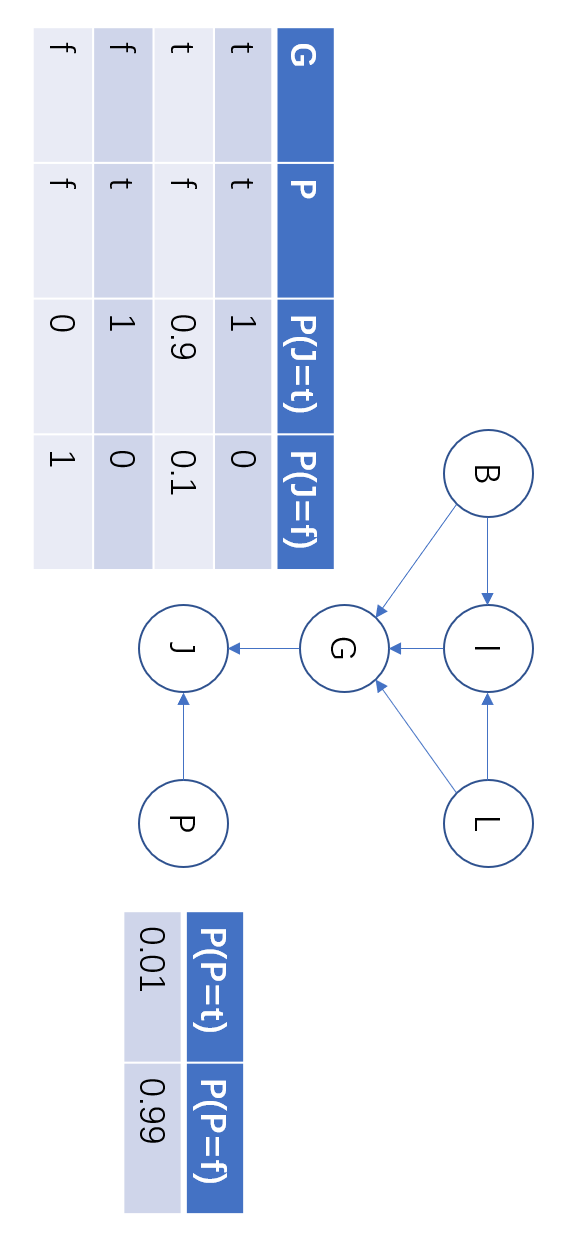
\includegraphics[width=0.5\linewidth]{Bayesian Brief Network.png}
\end{figure*}

\end{document}